\documentclass{article}
\usepackage[utf8]{inputenc}
\usepackage[margin=1in]{geometry}
\usepackage{graphicx}
\usepackage{caption}
\usepackage{subcaption}
\usepackage{cleveref}
\title{Sanity Checks for Saliency Maps}
\author{Alexander Haenel, Florian Kneifel, Lennart Rosseburg}
\date{July 2021}

\begin{document}

\maketitle

\section{Introduction}
Highlighting important features of the input data becomes more and more relevant when it comes to debugging or understanding learned models. Explanation methods are used as tools for this purpose inside environments where an input is considered to be relevant for the predictions of a learned model. Especially, \textit{saliency methods} have emerged as a popular class of tools designed to do that task of elucidating important aspects from an input, which is typically an image, and through that creating a so-called heat map. Based on their results, the individual decisions made by deep-learning models are tried to be explained. (Adebayo et al. 2018)\par 
As more contributions were made, a methodological challenge became clear: "\textit{the difficulty of assessing the scope and quality of model explanations}" (Adebayo et al. 2018). Adebayo et al. (2018) addressed this challenge, as they did not find it sufficient, but rather misleading, to rely solely on visual assessments. They showed with multiple experiments that several existing saliency methods are independent to both the model and the data generating process. As consequence, those methods are not suitable for tasks sensitive to either model or data, like finding outliers, etc. To approach this problem, and to properly evaluate explanation methods, a methodology based on statistical randomization tests was proposed. They compare the results from the natural experiment with results from two distinct instantiations of an randomized experiment. Their methodology can be thought of as a sanity check for saliency methods. (Adebayo et al. 2018)\par
The first instantiation is the \textit{model parameter randomization test}. Through comparison with the output of an randomly init. untrained network of the same architecture, this test checks if the saliency method depends on the learned parameters of the model. If so, the output should differ drastically between both cases. Otherwise, the saliency method is insensitive to the models properties. They also tested different randomization techniques. Those were: randomly re-initializing all weights completely or in cascading order(starting from the top layer) and independently randomizing a single layer at a time while keeping others fixed. (Adebayo et al. 2018)\par
The second test, \textit{the data randomization test}, compares two different results of a saliency method. Both on the same model and dataset, but one time the datasets labels are randomly permuted. This is done in order to test the sensitivity of the method to the relationship between instances and labels. So again, significant different outputs should be expected. Elsewise the saliency method is insensitive to relationships between instances and labels from the original data and thereby cannot explain mechanisms that depend on that. (Adebayo et al. 2018) \par

\section{Re-implement a sanity check using PyTorch (and Captum)}
For this and the following badges please refer to the \textit{src} and \textit{results} folder or to the notebook "SaliencyMapsCNN.ipynb".\\

We decided to re-implement the \textit{data randomization test}, or sanity check, from the paper. In this re-implementation we are reusing an CNN from one of our previous Exercises. The CNN architecture looks as follows: input $\to$ conv (3x3, 48) $\to$ ReLu $\to$ conv (3x3, 96) $\to$ ReLu $\to$ max-pool (2x2) $\to$ conv (3x3, 192) $\to$ ReLu $\to$ max-pool (2x2) $\to$ fully connected (64 units) $\to$ ReLu $\to$ fully connected (10 units). We train the model with the stochastic gradient descent (SGD) optimizer for 5 iterations while using an momentum of 0.9 on the CIFAR10 dataset. With the descried setup we achieved an average accuracy of 75\%.\\

\cref{fig:ig_normal,fig:ig_random_labels} shows our results obtained with the integrated gradients salicy method on one of the CIFAR10 images. It can be observed, that the saliency map trained with randomized labels differs strongly from the one trained correctly.

\begin{figure}[h!]
\centering
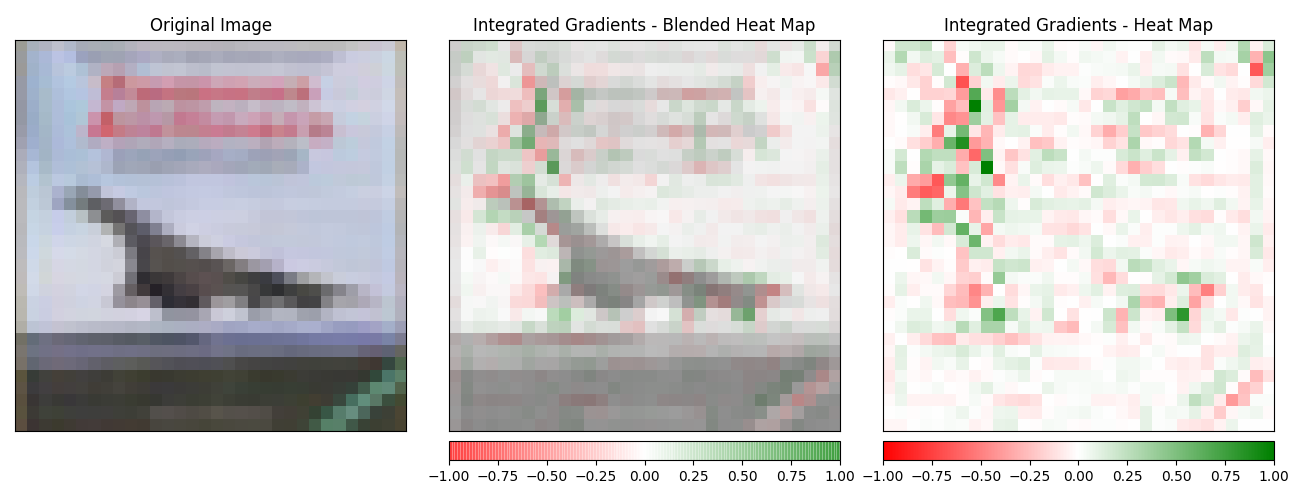
\includegraphics[width=\textwidth]{results/IG_normal.png}
\caption{Integrated Gradients}
\label{fig:ig_normal}
\end{figure}

\begin{figure}[h!]
\centering
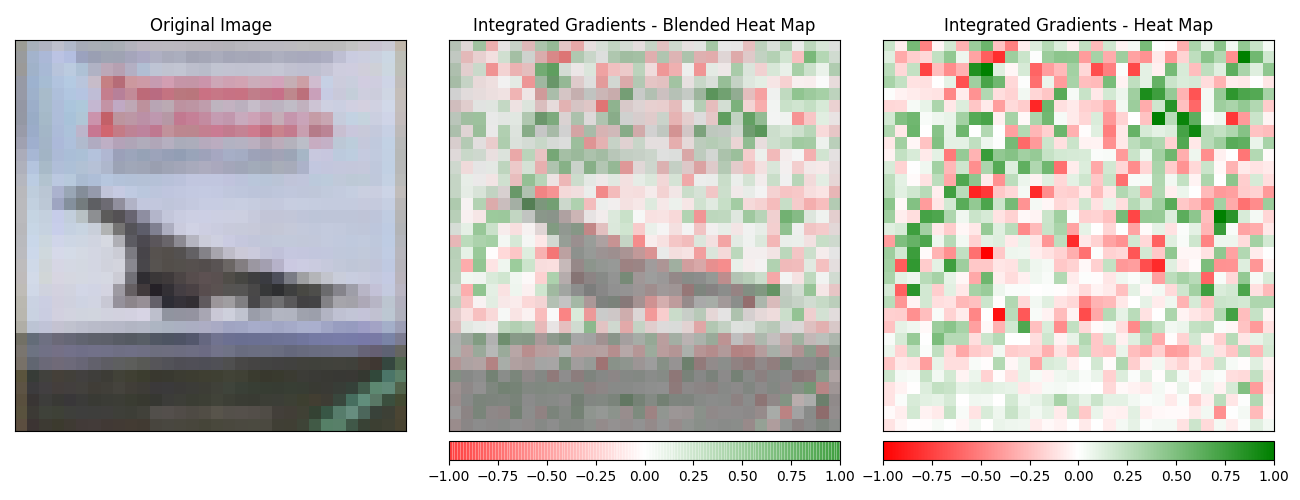
\includegraphics[width=\textwidth]{results/IG_random_labels.png}
\caption{Integrated Gradients with randomized labels}
\label{fig:ig_random_labels}
\end{figure}

\clearpage



\section{Experiment with different saliency methods}
Additionally to the integrated gradients saliency methods we also implemented DeepLift and an occlusion-based saliency method. From the figures below you can see that the saliency map generated from DeepLift is very simular to the one from integrated gradients, which also applies to the model trained on randomized labels. On the over hand the occlusion-based saliency map even on the correctly trained model looks a bit random and therefore there is no big difference to the model trained with randomized labels. The reason may be, that the model is not trained well enough with an accuracy of 75\%.\\

\cref{fig:dl_normal,fig:DL_random_labels,fig:occ_normal,fig:occ_random_labels} show our results obtained with the named salicy methods on one of the CIFAR10 images.

\begin{figure}[h!]
\centering
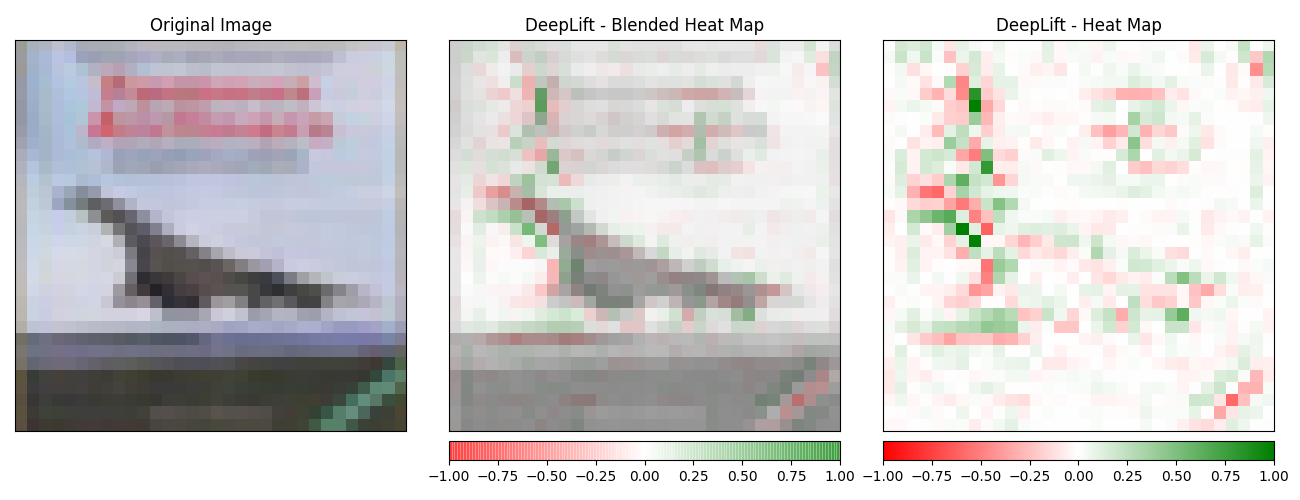
\includegraphics[width=\textwidth]{results/DL_normal.png}
\caption{DeepLift}
\label{fig:dl_normal}
\end{figure}

\begin{figure}[h!]
\centering
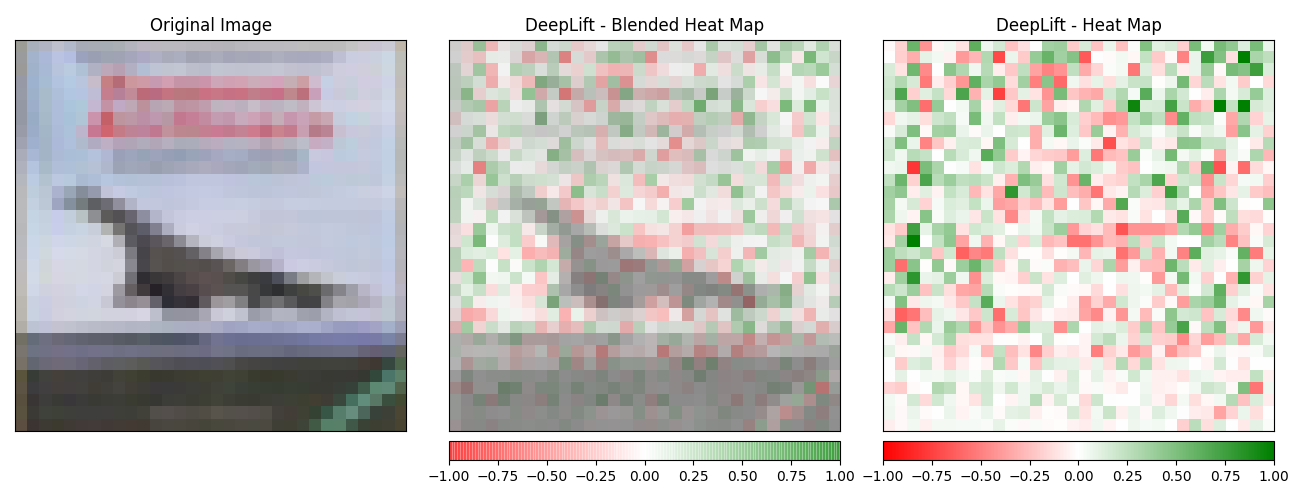
\includegraphics[width=\textwidth]{results/DL_random_labels.png}
\caption{DeepLift with randomized labels}
\label{fig:DL_random_labels}
\end{figure}

\begin{figure}[h!]
\centering
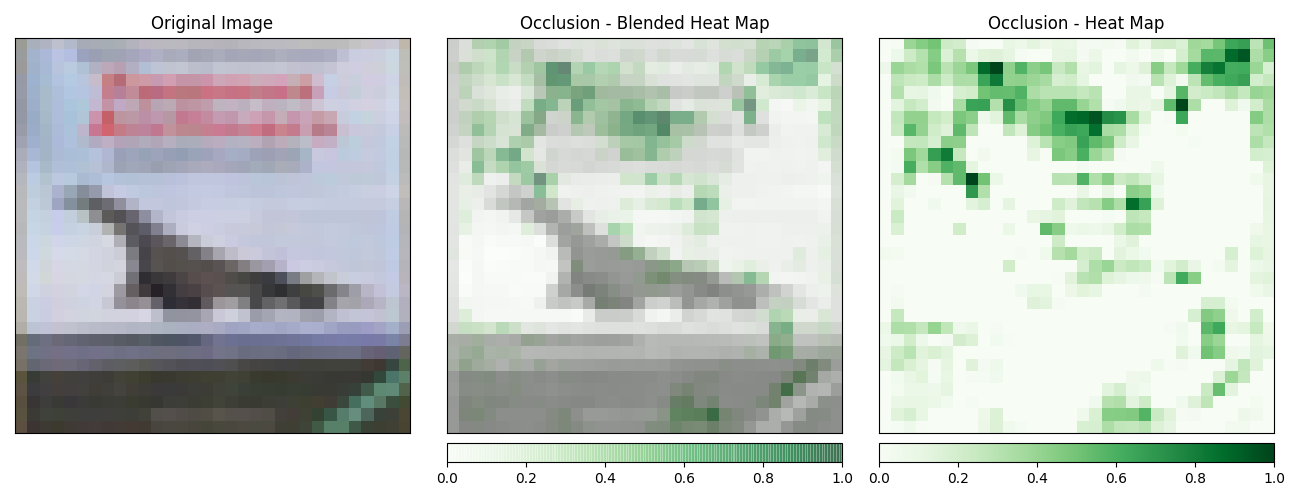
\includegraphics[width=\textwidth]{results/OCC_normal.png}
\caption{Occlusion-based saliency method}
\label{fig:occ_normal}
\end{figure}

\begin{figure}[h!]
\centering
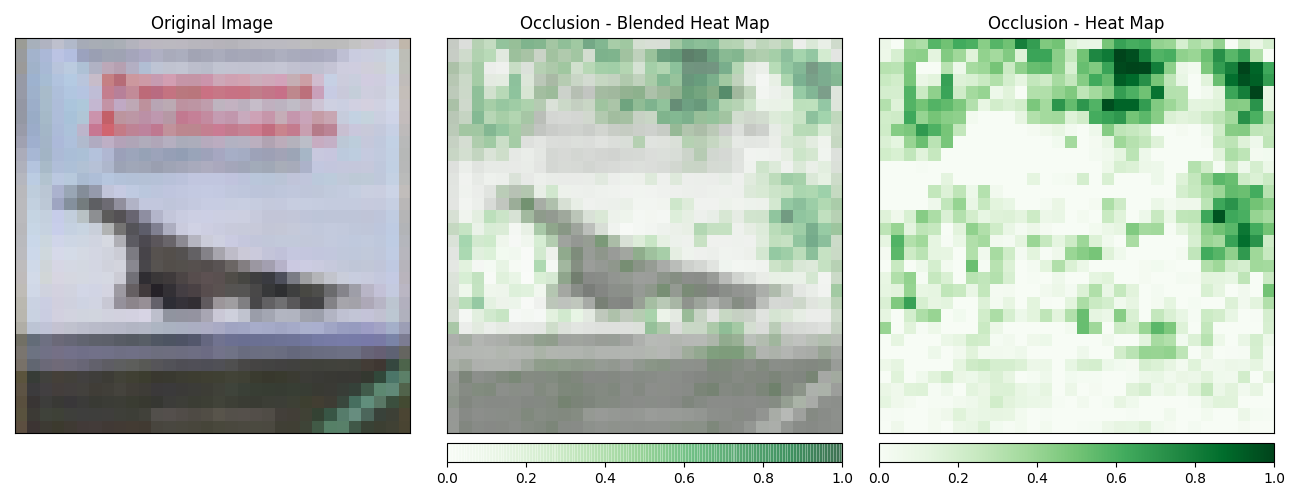
\includegraphics[width=\textwidth]{results/OCC_random_labels.png}
\caption{Occlusion-based saliency method with randomized labels}
\label{fig:occ_random_labels}
\end{figure}

\clearpage



\section{Run experiments on a different image classification dataset}
Instead of using the CIFAR10 dataset, we also tested the methods on the MNIST dataset. Since both datasets are structured equally, it was pretty easy to replace the dataset. Only two small adjustments where necessary. The input channels changed from three RGB channels for the CIFAR10 dataset to one input channel because of the gray-scale images on the MNIST dataset. Furthermore the number of neurons on the flattened linear layer changed, because of the different image sizes on CIFAR10 with 32x32 and on MNSIT with 28x28. 

Altogether we achieved an accuracy of 99\% with the described model. Somehow the captum module decided to show gray-scale images as purplish images but this shouldn't bother that much. \\

\cref{fig:MNIST_IG_normal,fig:MNIST_IG_random_labels} show our results obtained on one of the MNIST images with the integrated gradient saliency method. The saliency map is only visible where the number is actually written, because everywhere else the image is black (in the figures below purple) and therefore the input on these parts zero.

\begin{figure}[h!]
\centering
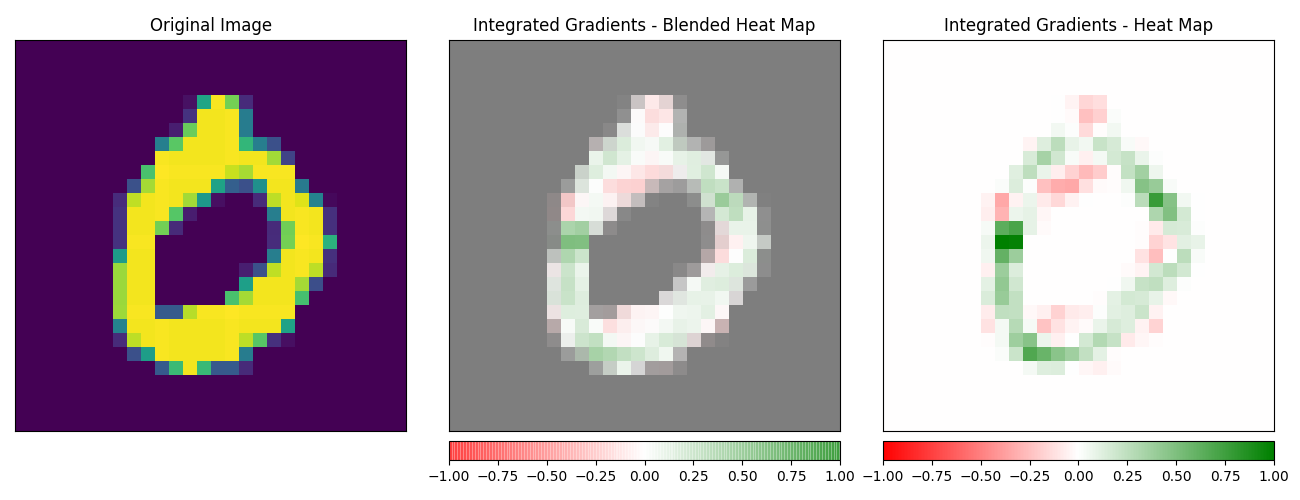
\includegraphics[width=\textwidth]{results/MNIST_IG_normal.png}
\caption{Integrated Gradients on an MNIST image}
\label{fig:MNIST_IG_normal}
\end{figure}

\begin{figure}[h!]
\centering
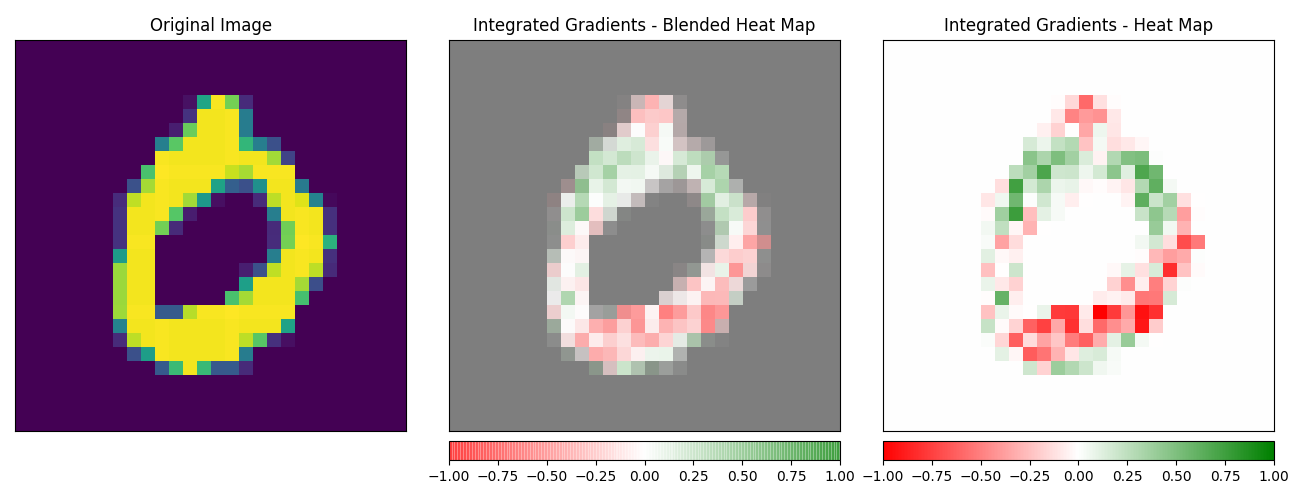
\includegraphics[width=\textwidth]{results/MNIST_IG_random_labels.png}
\caption{Integrated Gradients with randomized labels on an MNIST image}
\label{fig:MNIST_IG_random_labels}
\end{figure}

\clearpage



\section{Run experiments on non-image data}
For this badge please refer to the notebook "captum\textunderscore on\textunderscore timeseries.ipynb" 

\subsection{data}
As a simple toy-dataset for timeseries data, we use the "flights" dataset that comes with the seaborn library. The dataset contains the number of flight passengers per month for the years 1949 to 1960. So in total there are 144 datapoints. Just by looking at the data we can see a yearly pattern, but also a steady increase on a macro scale. Also for easier use the data in the notebook gets normalized before training a model. The task will be set up as a regression problem: The model gets the data from the last 10 months and has to predict the next month. Note that here we intentionally used a window smaller than 12, because otherwise the task will become to easy because of the intra-year-pattern.

\subsection{simple linear model}
For the first experiment we use a relatively simple linear model with the following architecture: 
\begin{itemize}
\item Input of size 10
\item Linear-Layer with 3 neurons
\item Sigmoid-Layer
\item Linear-Layer with 1 neuron
\end{itemize}
Considering the simplicity of the model, we get pretty accurate predictions:
\begin{figure}[h!]
\centering
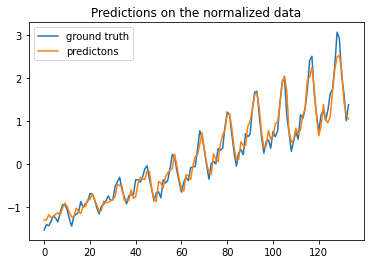
\includegraphics[scale=0.6]{results/linear_model_prediction.png}
\caption{linear model performance}
\label{fig:lin_model_perf}
\end{figure} \\
First we can look at which input feature on average has the most importance for the prediction:
\begin{figure}[ht!]
\centering
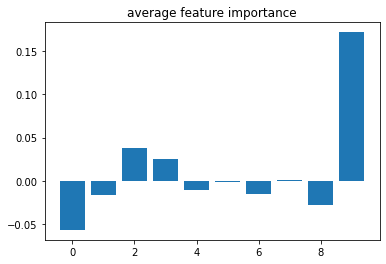
\includegraphics[scale=0.6]{results/linear_model_avg_feature_importance.png}
\caption{average feature importance}
\label{fig:lin_model_afi}
\end{figure} \\

There seems to be a pretty strong focus from the network towards the input at index 9. That is not surprising, considering that the number of flights most of the time is not drastically different from the last month. Looking at the average importance of neuron 0 in \ref{fig:lin_model_ani} and the negative correlation of almost every input for neuron 0 in \ref{fig:lin_model_anfi} one might conclude, that neuron 0 is trained to predict a decline, while neuron 1 and especially neuron 2 are mostly predicting increasing flight passengers.

\begin{figure}[h!]
     \centering
     \begin{subfigure}[b]{0.2\textwidth}
         \centering
         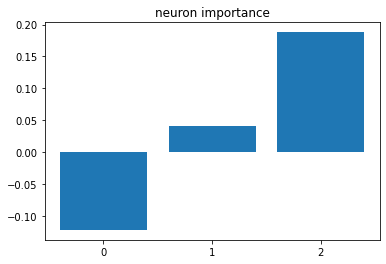
\includegraphics[scale=0.4]{results/linear_model_avg_neuron_importance.png}
         \caption{neuron importance}
         \label{fig:lin_model_ani}
     \end{subfigure}
     \hspace*{\fill}
     \begin{subfigure}[b]{0.4\textwidth}
         \centering
         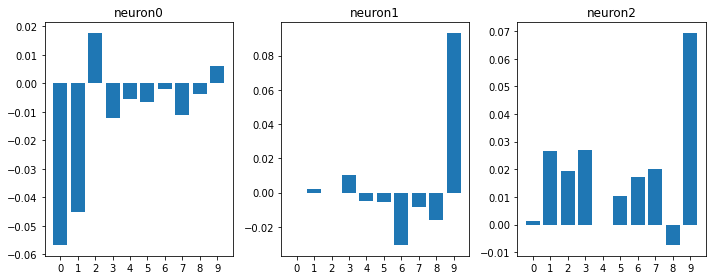
\includegraphics[scale=0.4]{results/linear_model_avg_feature_per_neuron_importance.png}
         \caption{average feature importance per neuron}
         \label{fig:lin_model_anfi}
     \end{subfigure}
     \hspace*{\fill}
        \caption{average importance}
        \label{fig:lin_model_a_f_i}
\end{figure}

\subsubsection{Pattern recognition}
Because of the way the data is organized, we can use a step size of 12 to get the same month for consecutive years. At first sight, we might assume that there is a certain regularity in the way the inputs are interpreted. But if we use a random model to repeat the same experiment, we see similar patterns emerging. (however because the attributions are way smaller a factor 10 is added to the visualization) In conclusion, we can not really get any insight in the pattern recognition performed by the neural network from this experiment.

For the last experiment we use a CNN to better resemble an architecture, that one would also find for image tasks. Just comparing the different methods provided by Captum shows quite different results. Especially looking at the input at index 9 shows a strong positive signal from the method "saliency" but is negative for "integrated gradients" and "deep lift".

All in all it is interesting to see which neuron behaves which way, and how the input features are correlated to the output. However interpreting the workings of the neural net from this information is not possible. For this timeseries-task it is even harder, because even with a lot of training we as humans can not simply look at a short timeseries plot and predict the next value. At picture classification humans are naturally gifted and can generally perform well.

\end{document}